\documentclass[10pt,twocolumn,letterpaper]{article}
\usepackage[italian]{babel} 
\usepackage[utf8]{inputenc} 
\usepackage{cvpr}
\usepackage{times}
\usepackage{epsfig}
\usepackage{graphicx}
\usepackage{amsmath}
\usepackage{amssymb}
\usepackage{url}

% Include other packages here, before hyperref.

% If you comment hyperref and then uncomment it, you should delete
% egpaper.aux before re-running latex.  (Or just hit 'q' on the first latex
% run, let it finish, and you should be clear).
%\usepackage[pagebackref=true,breaklinks=true,letterpaper=true,colorlinks,bookmarks=false]{hyperref}

\cvprfinalcopy % *** Uncomment this line for the final submission

\def\cvprPaperID{****} % *** Enter the CVPR Paper ID here
\def\httilde{\mbox{\tt\raisebox{-.5ex}{\symbol{126}}}}

% Pages are numbered in submission mode, and unnumbered in camera-ready
\ifcvprfinal\pagestyle{empty}\fi
\begin{document}

%%%%%%%%% TITLE
\title{Clustering di immagini basato su Normalized Cuts per l'identificazione di camera}

\author{Lorenzo Cioni\\
{\tt\small lore.cioni@gmail.com}
% For a paper whose authors are all at the same institution,
% omit the following lines up until the closing ``}''.
% Additional authors and addresses can be added with ``\and'',
% just like the second author.
% To save space, use either the email address or home page, not both
\and
Saverio Meucci\\
{\tt\small s.meucci91@gmail.com}
}

\maketitle
\thispagestyle{empty}

%%%%%%%%% ABSTRACT
\begin{abstract}

L'obiettivo di questo elaborato è di implementare un sistema di identificazione di camera basato sul clustering di immagini in gruppi eterogenei, utilizzando come distanza la \emph{PCE}, \emph{peaks-to-correlation energy ratio}, tra i PRNU delle immagini. L'algoritmo di clustering implementato è \emph{Normalized Cuts}.

Una volta creati i gruppi di immagini, per ciascuno di essi verrà estratta la PRNU di camera e sarà dunque possibile comparare una nuova immagine per stabilire a quale camera appartiene.

Per validare il metodo implementato sono proposti diversi risultati sperimentali basati su dataset differenti. Uno degli o
\end{abstract}



%-------------------------------------------------------------------------
\section{Introduzione}

Il problema dell'identificazione della fotocamera digitale da cui una foto è stata scattata è un problema noto dell'\emph{image forensics}. 

Descrizione generale del problema: citare articolo, l'implementazione parte da quello.

Come funziona: step dell'algoritmo

1. estrazione prnu e calcolo pce
2. clustering 
3. fingerprint
4. validazione risultati

(citare relative sezioni)

Linguaggio usato
\section{Il \emph{pattern noise}}

Durante tutto il processo di acquisizione ed elaborazione, l'immagine può essere affetta da rumore. 
In particolare, ogni fotocamera digitale possiede un sensore
lievemente differente dalle altre dello stesso modello, per via di un \emph{disturbo}
univoco e riconoscibile, ciò permette di identificare il sensore a partire dalle
immagini, sfruttando lo stesso principio della balistica nel riconoscimento dei segni lasciati dai proiettili nelle armi.

Il disturbo generato nelle immagini è legato sia al sensore che ai dettagli costruttivi. Questo
assicura una differenza tra singoli dispositivi sufficiente a rendere improbabile
la presenza di due camere che generino il medesimo disturbo, proprio come avviene per le impronte digitali. 

Rumori di questo genere sono di tipo \emph{pattern noise}. Quest'ultimo è composto da due parti: il \emph{Fixed Pattern Noise} (FPN) ed il rumore \emph{Photo-Response Non-Uniformity} (PRNU).

FPN è un rumore casuale e può essere automaticamente rimosso sottraendo all'immagine originale un'immagine scura. Anche il PRNU può essere scomposto nel rumore \emph{Pixel Non-Uniformity} (PNU) e componenti a bassa frequenza, dove il PNU è il risultato della differenza di luminosità dei pixel a causa delle regioni non omogene del sensore e delle imperfezioni nella costruzione dello stesso.

Due immagini acquisite dallo stesso sensore CCD generalmente presentano lo stesso rumore PNU; inoltre il PNU non è soggetto a variazioni di temperatura o umidità il che lo rende adatto allo scopo dell'identificazione della sorgente.

Il rumore residuo di un'immagine $W$ può essere espresso come
$$
W = I - F(I) = IK - \Xi
$$
dove $F()$ è una funzione di \emph{denoising}, $K$ è una costante e $\Xi$ è un insieme di fattori di rumore.

A questo punto è necessario stimare $K$ a partire da un insieme $N$ di immagini ottenute dalla medesima camera, assumendo che $\Xi$ sia di tipo gaussiano. Per ciascun $k = 1, \ldots, N$:
$$
\frac{W_k}{I_k} = K + \frac{\Xi_k}{I_k}
$$
La \emph{log-likelihood} di $\frac{W_k}{I_k}$, dato $K$, è calcolata con
$$
L(K) = -\frac{N}{2} \sum_{k = 1}^{N} log(\frac{2\pi\sigma^2}{I_{k}^{2}}) -  \sum_{k = 1}^{N} \frac{(W_k / I_k - K)^2}{2\sigma^2 / I_{k}^{2}}
$$
Si risolve l'equazione $\frac{\delta L(K)}{\delta K} = 0$ per ottenere la stima $\hat{K}$ di $K$:
$$
\hat{K} = \frac{\sum_{k = 1}^{N} W_k I_k}{\sum_{k = 1}^{N} I_{k}^{2}}
$$



cosa è il prnu in generale (non nel dettaglio) e come si calcola la pce tra due prnu

dettagli della estrazione: resize immagini (alla dimensione inferiore), rotazione immagini in landscape mode
\section{Clustering}

Il metodo di identificazione di dispositivi ignoti a partire da un'insieme di immagini digitali campione prevede una fase di clustering che, usando la PRNU di ciascuna immagine, va a suddividere tale insieme in un sotto insieme di immagini simili, ovvero con lo stesso pattern noise e quindi, presumibilmente, provenienti dallo stesso sensore.
L'insieme delle PRNU delle immagini viene rappresentato con un grafo pesato completamente connesso, in cui le PRNU, e quindi le immagini, rappresentano i nodi. I pesi associati a ciascun arco sono calcolati con la PCE (Peak-to-Correlation Energy), una misura di similarità che si adatta molto bene per le fingerprint, calcolate con la PRNU, di immagini bidimensionali. La caratteristica principale di tale misura è che la presenza di pattern periodici nascosti diminuisce la PCE. Quindi il peso associato all'arco sarà tanto più alto quanto più i nodi interessati avranno una PRNU simile. Il grafo pesato può essere rappresentato da una matrice quadrata $N\times N$, con N numero di immagini.
Calcolare la PCE per tutti i nodi del grafo è una delle operazioni più costose del metodo di identificazione implementato, infatti calcolare la matrice dei pesi ha complessità quadratica con il numero di immagini.

Una volta costruito il grafo pesato possiamo procedere con la fase di clusterizzazione, per suddividere le immagini in gruppi di immagini simili, in base alla loro PRNU.


\subsection{Normalized Cuts}

Dato una grafo $ G = <V, E> $, gli archi $E$ che connettono ciascuna coppia di nodi, ovvero di PNRU, sono pesati con la PCE, come descritto in precedenza, dove $PCE(i, j)$ rappresenta la similarità fra il nodo $i$ e il nodo $j$.
L'algoritmo di clusterizzazione Normalized Cuts è un algoritmo ricorsivo, che ad ogni iterazione, bipartiziona il grafo G, creando quindi due sottografi A e B ($A\cup B = V$ e $A\cap B = \emptyset$). Una volta ottenuti due sottografi è possibile dare un valore del taglio, ovvero calcolare il peso totale  degli archi rimossi che fornisce una stima sul grado di dissimilarità di questi due sottografi. Il taglio è calcolato come segue: 

\begin{equation}
cut(A,B) = \sum_{u\in A, v\in B} w(u, v)
\end{equation}

Il taglio ottimale per bipartizionare il grafo è calcolato ottimizzando il valore di un taglio normalizzato, ideato dagli autori originali dell'algoritmo per evitare che si favorisca la creazione di piccoli cluster composti da nodi isolati. Il taglio normalizzato, da cui l'algoritmo Normalized Cuts prende il nome, è calcolato come segue: 
\begin{equation}
Ncut(A,B) =  \frac{cut(A,B)}{assoc(A,V)} + \frac{cut(A,B)}{assoc(B,V)}
\end{equation}
dove $assoc(A,V) = \sum_{u\in A, t\in V} w(u,t) $ rappresenta la somma dei pesi degli archi che connettono i nodi della partizione A ad un generico nodo del grafo G.
Va notato che la misura di $cut(A,B)$ è sempre minore di $assoc(A,V)$ e di $assoc(B,V)$. Gli archi che sono rimossi sono una frazione degli archi che hanno un nodo in A e l'altro nodo in B. Il valore $assoc(A,V) - cut(A,B)$ misura la somma dei pesi degli archi che collegano due nodi in A. Quindi, il valore di $ \frac{cut(A,B)}{assoc(A,V)}$ è basso quando i nodi in A hanno un grado di similarità fra di loro e un basso grado di similarità con in nodi che non appartengono ad A. Il taglio normalizzato ha quindi la proprietà di partizionare il grafo in due segmenti A e B tale che la somma dei pesi degli archi che connettono le due partizioni è bassa.

Per calcolare il taglio normalizzato ottimale, occorre:
\begin{itemize}
\item una matrice dei pesi, calcolata nel nostro caso con la PCE, che rappresenta la similarità fra ciascun nodo.
\item un vettore di componenti $\gamma$, che rappresenta il taglio, di dimensione pari al numero di nodi del grafo. Il valore dell'i-esimo componente è pari a 1 se l'i-esimo nodo appartiene al primo segmento; è pari a 0 se l'i-esimo nodo appartiene alla seconda partizione.
\item una degree matrix $D = \lbrace d_{ii} \rbrace $, una matrice diagonale, in cui ogni elemento che è sulla diagonale è la somma di tutti i pesi degli archi che partono dall'i-esimo nodo, ovvero $d_{ii} = \sum_{j} a_{ij}$
\end{itemize}

Può essere dimostrato che il taglio che minimizza il costo normalizzato, minimizza anche la seguente funzione: \begin{equation}
\frac{\gamma^{T}(D-A)\gamma}{\gamma^{T}D\gamma}
\end{equation}
La soluzione $\gamma$, che rappresenta il taglio, dovrebbe essere un vettore di valori discreti in $\lbrace 0,1 \rbrace$. Tale funzionale è una versione discreta del quoziente di Rayleigh. Risolvere tale funzionale per valori discreti è un problema NP-completo. Tuttavia, il problema diventa trattabile se la soluzione $\gamma$ è libera di assumere valori reali. A questo punto, minimizzare il costo di una funzione per un vettore $\gamma$ di valori reali è equivalente alla soluzione della seguente equazione: 
\begin{equation}
(D-A) \gamma = \lambda D \gamma
\end{equation}
Poichè il più piccolo autovalore di $(D-A)$ è pari a zero, può essere dimostrato che la soluzione all'equazione è l'autovettore corrispondente al secondo più piccolo autovalore.
Una volta ottenuta la soluzione reale è necessario discretizzarla nei valori $\lbrace 0,1 \rbrace$. Occore quindi scegliere un valore di soglia. Per fare ciò si può utilizzare il valore 0 o il valore mediano fra gli elementi della soluzione come valore di soglia oppure si può scegliere il valore, fra gli elementi della soluzione, che minimizza il valore di $Ncut(A,B)$.

La procedura di bipartizione del grafo può essere riassunta come segue:
\begin{enumerate}
\item Dato un insieme di features, costruire un grafo pesato $G = <V,E>$, calcolando i pesi di ciascun arco che rappresentano una similarità fra i nodi.
\item Risolvere l'equazione mostrata precedentemente Eq.(8) utilizzando l'autovettore corrispondente al secondo più piccolo autovalore.
\item Usare tale soluzione per bipartizionare il grafo, in modo tale che il costo del taglio normalizzato sia minimo.
\item Decidere se le due partizione correnti devono essere suddivise ricorsivamente andando a calcolare una misura della stabilità del taglio.
\end{enumerate}

Nella seguente sottosezione verrà spiegato in maggiore dettaglio lo step 4.

\subsubsection{Soglie}

L'algoritmo Normalized Cuts si basa su uno step ricorsivo che dipende dalla verifica di stabilità del taglio appena realizzato. L'implementazione originale dell'algoritmo prevede di comparare il valore di $Ncut(A,B)$ ad una soglia $T_{k}$ decisa a priori. Gli autori di \cite{ Amerini2014831} hanno invece definito un coefficiente di aggregazione, $AC(k) = \frac{1}{N_{k}} \sum_{i,j} w(i,j)$, ovvero il valore medio dei pesi associati ai nodi che appartengono alla partizione $k$, calcolato per ciascuna partizione ottenuta; se tale valore è minore di una soglia $T_{k}$ predefinita la partizione viene ulteriormente suddivisa, se è maggiore la ricorsione si ferma.

Per decidere quali dei due metodi usare nella nostra implementazione e quale soglia $T_{k}$ predefinita utilizzare, è stato usato un approccio basato su curve ROC prendendo come parametri di correttezza della clusterizzazione il valori di TPR e FPR rispetto ad un ground-truth. Per fare ciò abbiamo considerato un sottoinsieme di 20 immagini da ciascun dispositivo del dataset utilizzato, in modo da considerare tutti i dispositivi in nostro possesso per la scelta della soglia $T_{k}$.

Il range di variazione della soglia $T_{k}$ differisce a seconda del metodo utilizzato, ovvero il valore di $Ncut$ o il coefficiente di aggregazione. I grafici mostrati in seguito rappresentano l'andamento dei valori di TPR e FPR al variare della soglia. Tali esperimenti sono stati fatti sia per le immagini direttamente acquisite dai dispositivi, sia per le immagini caricate e riscaricate da Facebook, con l'opzione per il download ad alta risoluzione.

\begin{figure}[h]
\begin{center}
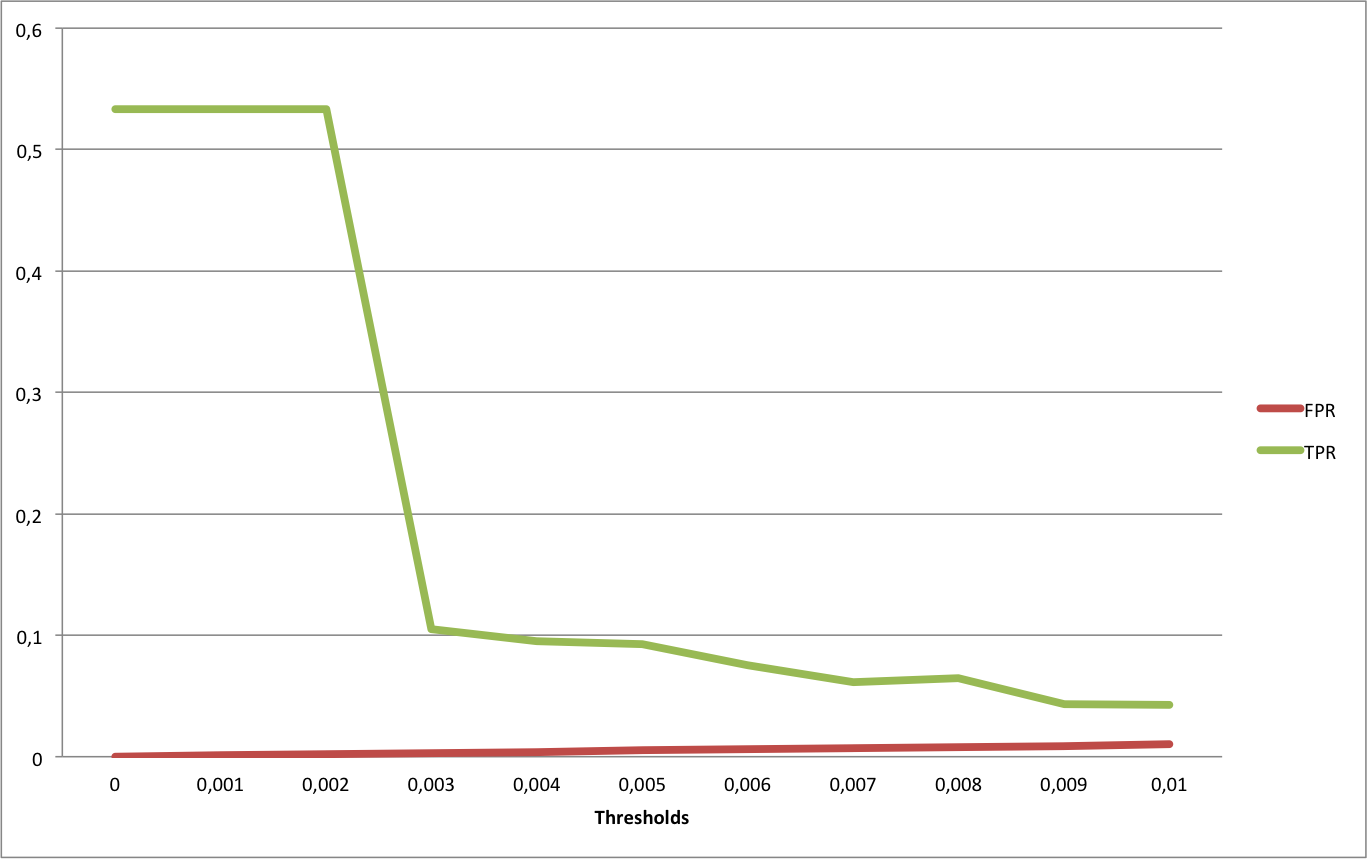
\includegraphics[width=0.4\textwidth]{images/soglia_imgnat_AC.png}
\end{center}
  \caption{Valori di TPR e FPR al variare della soglia per le immagini naturali acquisite direttamente dai dispositivi. Metodo con coefficiente di aggregazione.}
\label{fig:soglia AC}
\end{figure}

\begin{figure}[h]
\begin{center}
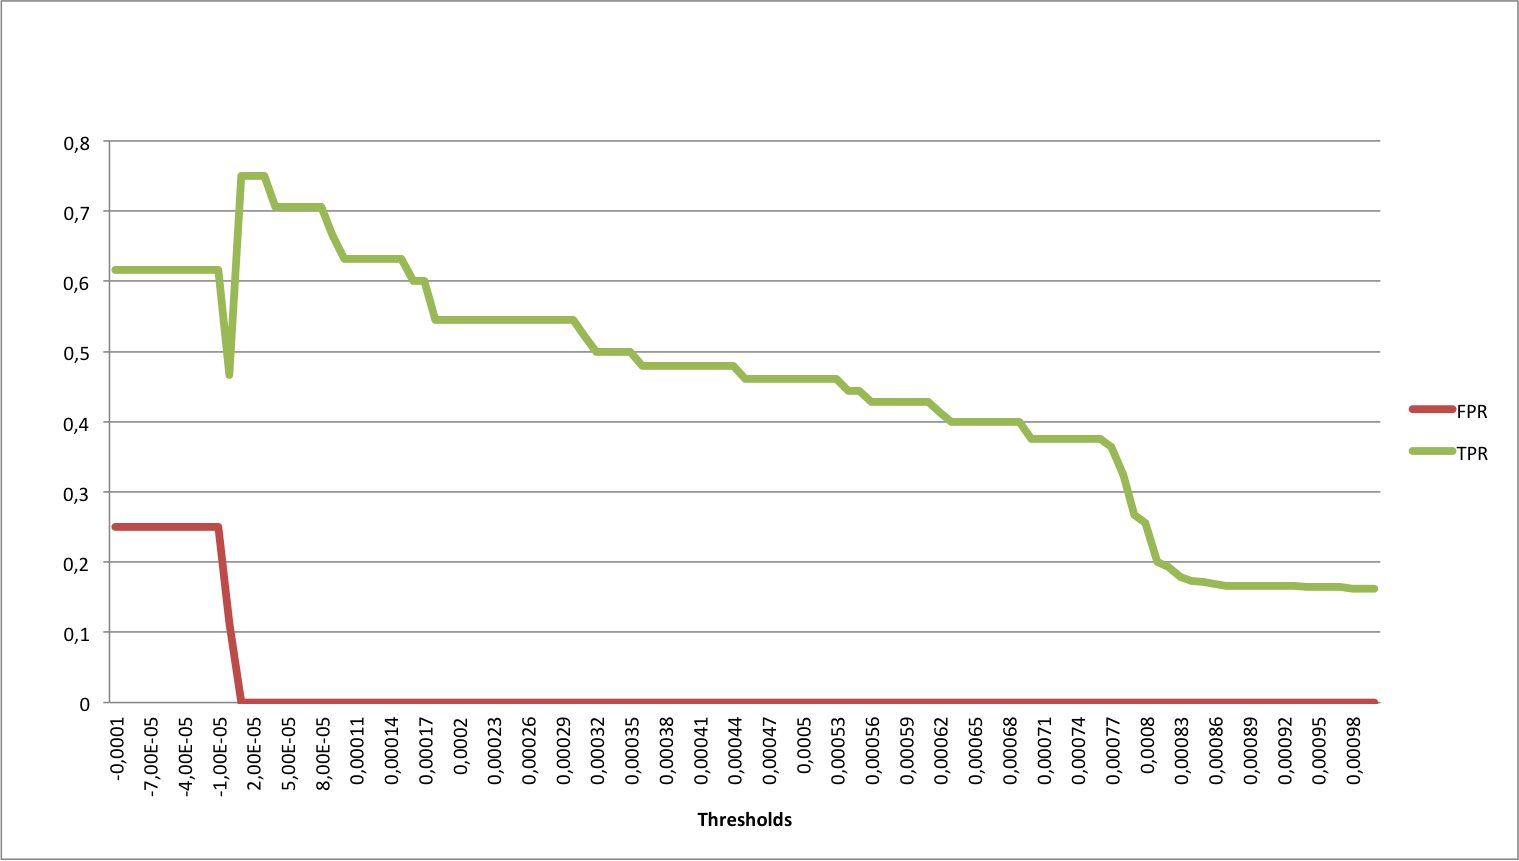
\includegraphics[width=0.4\textwidth]{images/soglia_imgnat_NC.png}
\end{center}
  \caption{Valori di TPR e FPR al variare della soglia per le immagini naturali acquisite direttamente dai dispositivi. Metodo che considera i valori di $Ncuts$.}
\label{fig:soglia AC}
\end{figure}

\begin{figure}[h]
\begin{center}
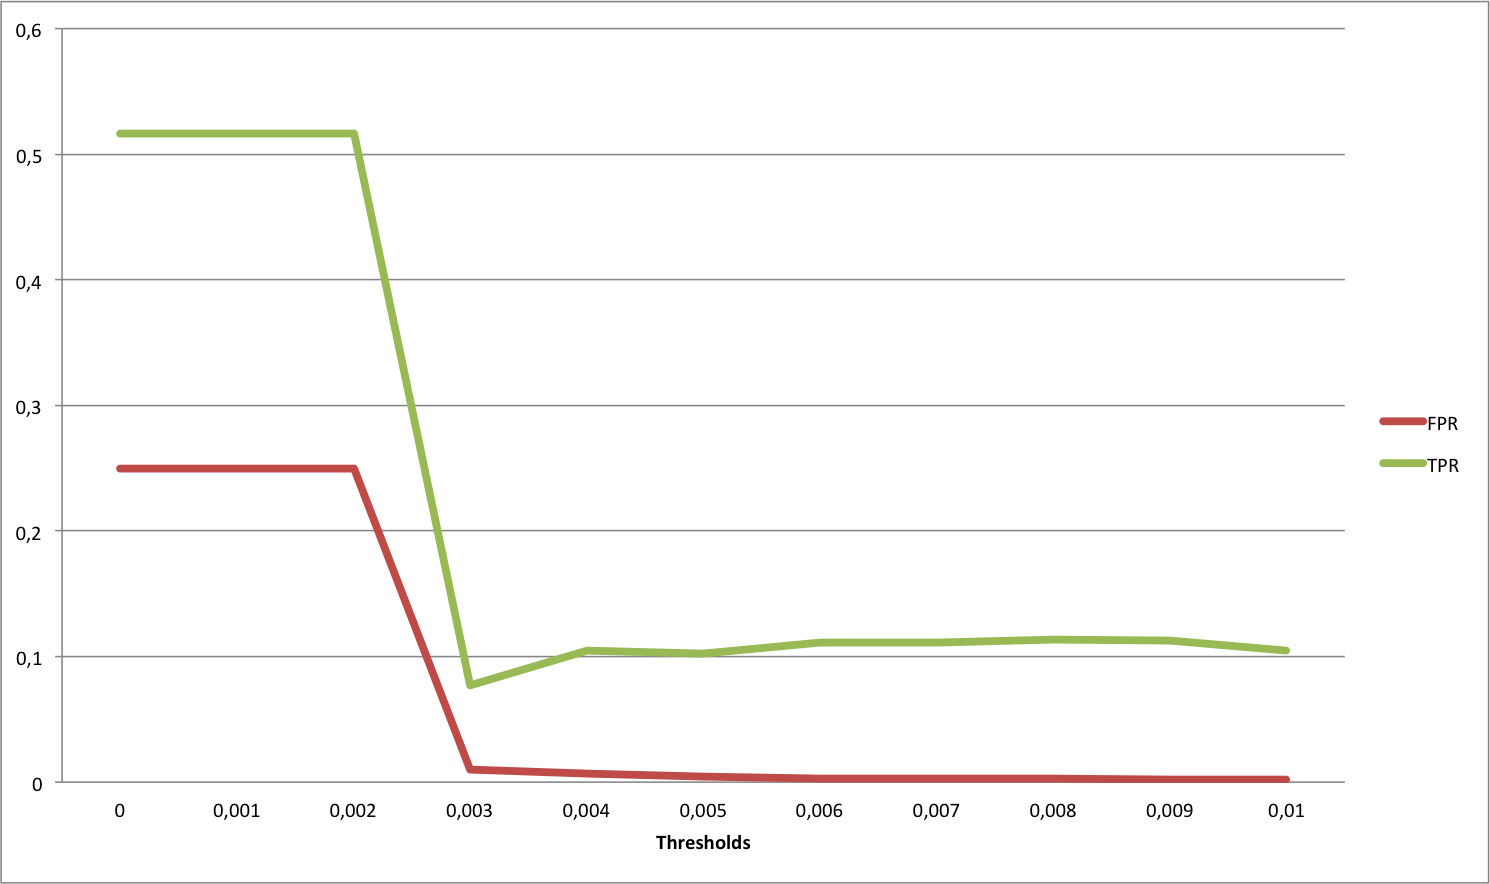
\includegraphics[width=0.4\textwidth]{images/soglia_imgnat_fb_AC.png}
\end{center}
  \caption{Valori di TPR e FPR al variare della soglia per le immagini scaricate da Facebook. Metodo con coefficiente di aggregazione.}
\label{fig:soglia AC}
\end{figure}

\begin{figure}[h]
\begin{center}
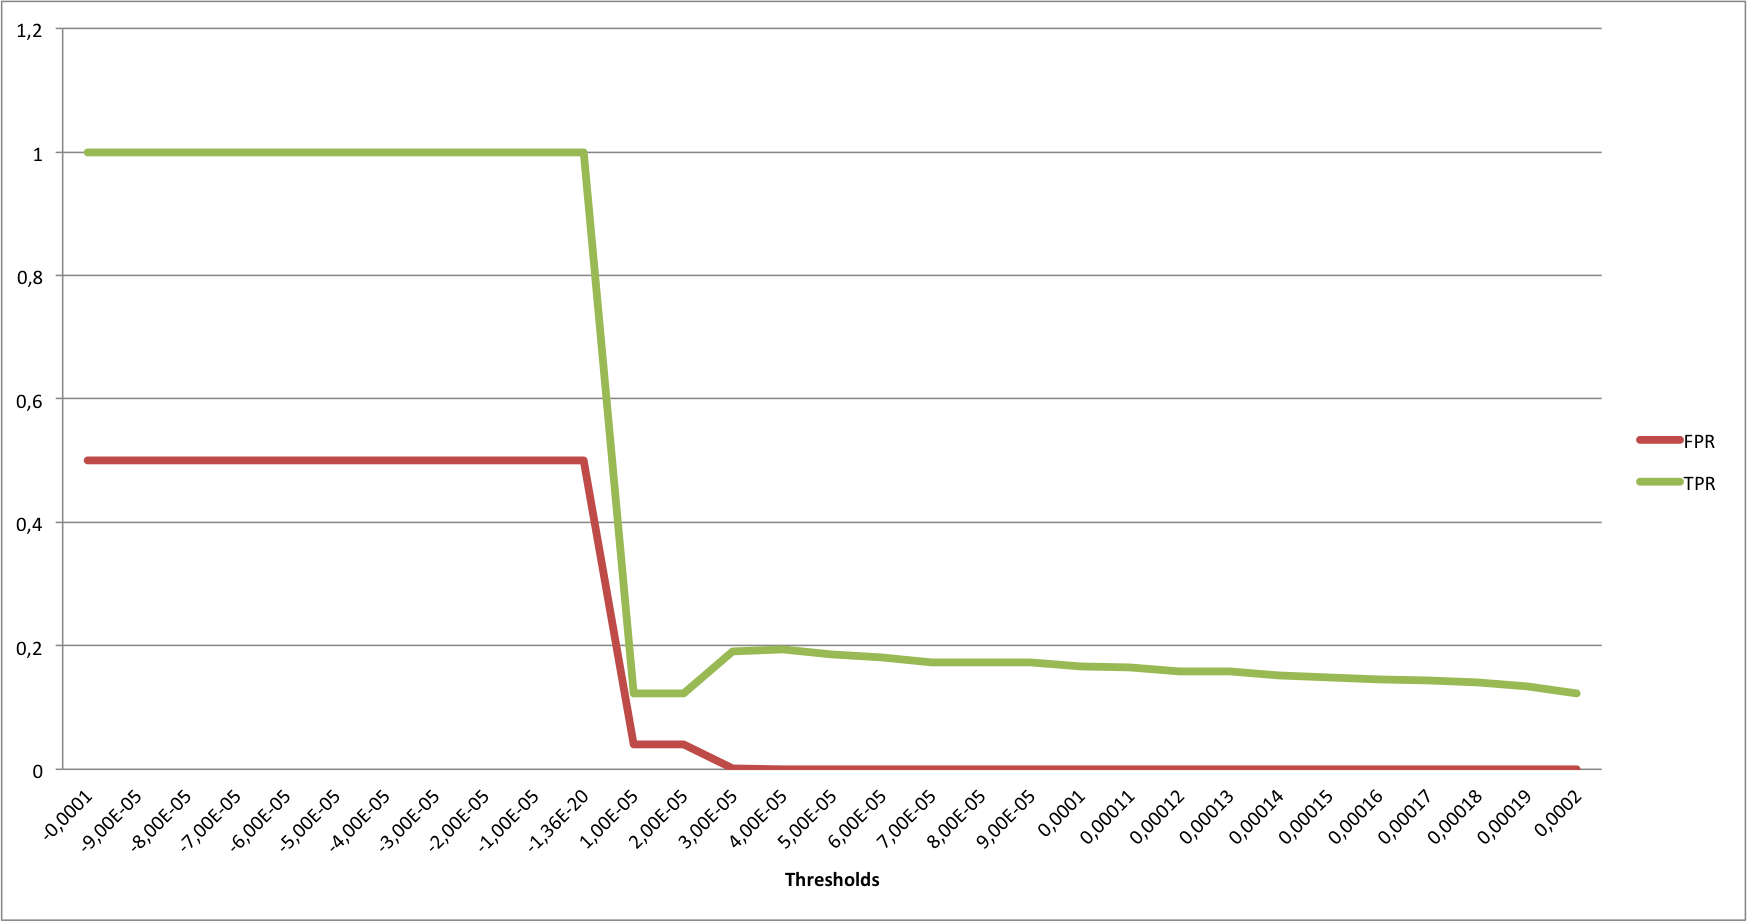
\includegraphics[width=0.4\textwidth]{images/soglia_imgnat_fb_NC.png}
\end{center}
  \caption{Valori di TPR e FPR al variare della soglia per le immagini scaricate da Facebook. Metodo che considera i valori di $Ncuts$.}
\label{fig:soglia AC}
\end{figure}

Nella nostra implementazione, come si può notare dai risultati, il metodo che utilizza $Ncut$ risulta essere il migliore quando vengono usate le immagini direttamente acquisite dai dispositivi. Per questo caso è stata selezionata come migliore soglia $T_{k} = 10^{-5}$ che corrisponde al valore massimo di TPR, pari a 0.75, e al valore minimo di FPR, pari a 0; ciò significa che le immagini non sono perfettamente raggruppate, ovvero il numero di clusters è maggiore di quello atteso, ma al contempo i clusters ottenuti sono "puliti", ovvero sono composti solo da elementi simili, non contengono, cioè, falsi positivi.
Per il caso delle immagini provenienti da Facebook, il confronto fra i due metodi è più incerto. Ciò è probabilmente dovuto al fatto che, subendo una compressione, la PRNU di tali immagini perde informazione in grado di discriminarle a sufficienza. Infatti i risultati ottenuti mostrano un numero significativo di falsi positivi contenuti nei clusters in entrambi i metodi, una situazione non desiderabile poichè è a partire da tali clusters che verranno calcolate le fingerprints relative ai dispositivi. Inoltre i minimi valori di FPR si ottengono in corrispondenza dei minimi valori di TPR; ciò indica che i clusters ottenuti sono perlopiù cluster singoli o con pochi elementi, altro caso non desiderabile. Tuttavia, per coerenza con il caso precendente, è stata scelto di utilizzare il metodo relativo a $Ncuts$, poichè mostra più consistenza con il valore ottimale della soglia $T_{k}$ del caso precedente, questa volta pari a $4*10^{-5}$ e che corrisponde al valore minimo di FPR.

In generale la scelta della soglia ottimale è stata fatta minimizzando il valore dei falsi positivi all'interno dei clusters calcolati; è preferibile ottenere più clusters ma che genereranno fingerprints senza rumore, piuttosto che un numero esatto di clusters da cui però si otterranno fingerprints rumorose.

\section{Estrazione delle \emph{fingerprint}}
\section{Validazione}
\section{Esperimenti}

\subsection{Dataset}

Per gli esperimenti è stato utilizzato un dataset che contiene un totale di 14 dispositivi, che includono smartphone e tablet, di diverse case produttrici e modelli. In particolare i modelli in nostro possesso sono: un Galaxy S3, due Galaxy S3 mini, un Galaxy S4 mini, un Galaxy Tab 3, un Galaxy Tab, un Galaxy Trend Plus, un Huawei G6, un Ipad 2, un Ipad mini, un Iphone 4S, un Iphone 5C, un Iphone 5 e un Iphone 6. Di tutti questi dispositivi siamo in possesso di immagini direttamente acquisite (immagini naturali) e delle stesse immagini ma caricate e scaricate da Facebook, in particolare ci siamo concentrati sulle immagini scaricate da Facebook in alta risoluzione.

La fase di estrazione delle fingerprint è stata eseguita tre volte con tre diversi sottoinsieme del dataset di dimensione differente. In particolare, seguendo gli esperimenti di [cit] sono stati usati insiemi da 6 dispositivi (un Galaxy S3, due Galaxy S3 mini, un Galaxy S4 mini, un Galaxy Tab 3, un Galaxy Tab), 5 dispositivi (un Huawei G6, un Ipad 2, un Ipad mini, un Iphone 4S, un Iphone 5C) e 4 dispositivi (un Galaxy Tab 3, un Galaxy Tab, un Galaxy Trend Plus, un Huawei G6). Dai dispositivi sono state selezionate 50 immagini, per un totale di 300, 250, 200 immagini rispettivamente per i tre casi.

Come spiegato in precedenza, la fase di validazione consiste nel verificare se sono state calcolate delle buone fingerprint, ovvero che siano in grado, data una generica immagine appartente al dataset non usata in precedenza, di assegnarle il giusto dispositivo. In questa fase le camere sono state suddivise in gruppi uguali alla fase di estrazione delle fingerprint, utilizzando però 20 immagini da ciascun dispositivo non usate nella fase precedente.

\subsection{Risultati}

I risultati sono molto diversi per il caso delle immagini naturali e per il caso delle immagini di Facebook in alta risoluzione. Tali risultati sono ottenuti utilizzando le modalità descritte in precedenza, ovvero Normalized Cuts con $Ncuts$ come condizione di stop con soglia pari a $10^{-5}$.

\begin{figure}[h]
\begin{center}
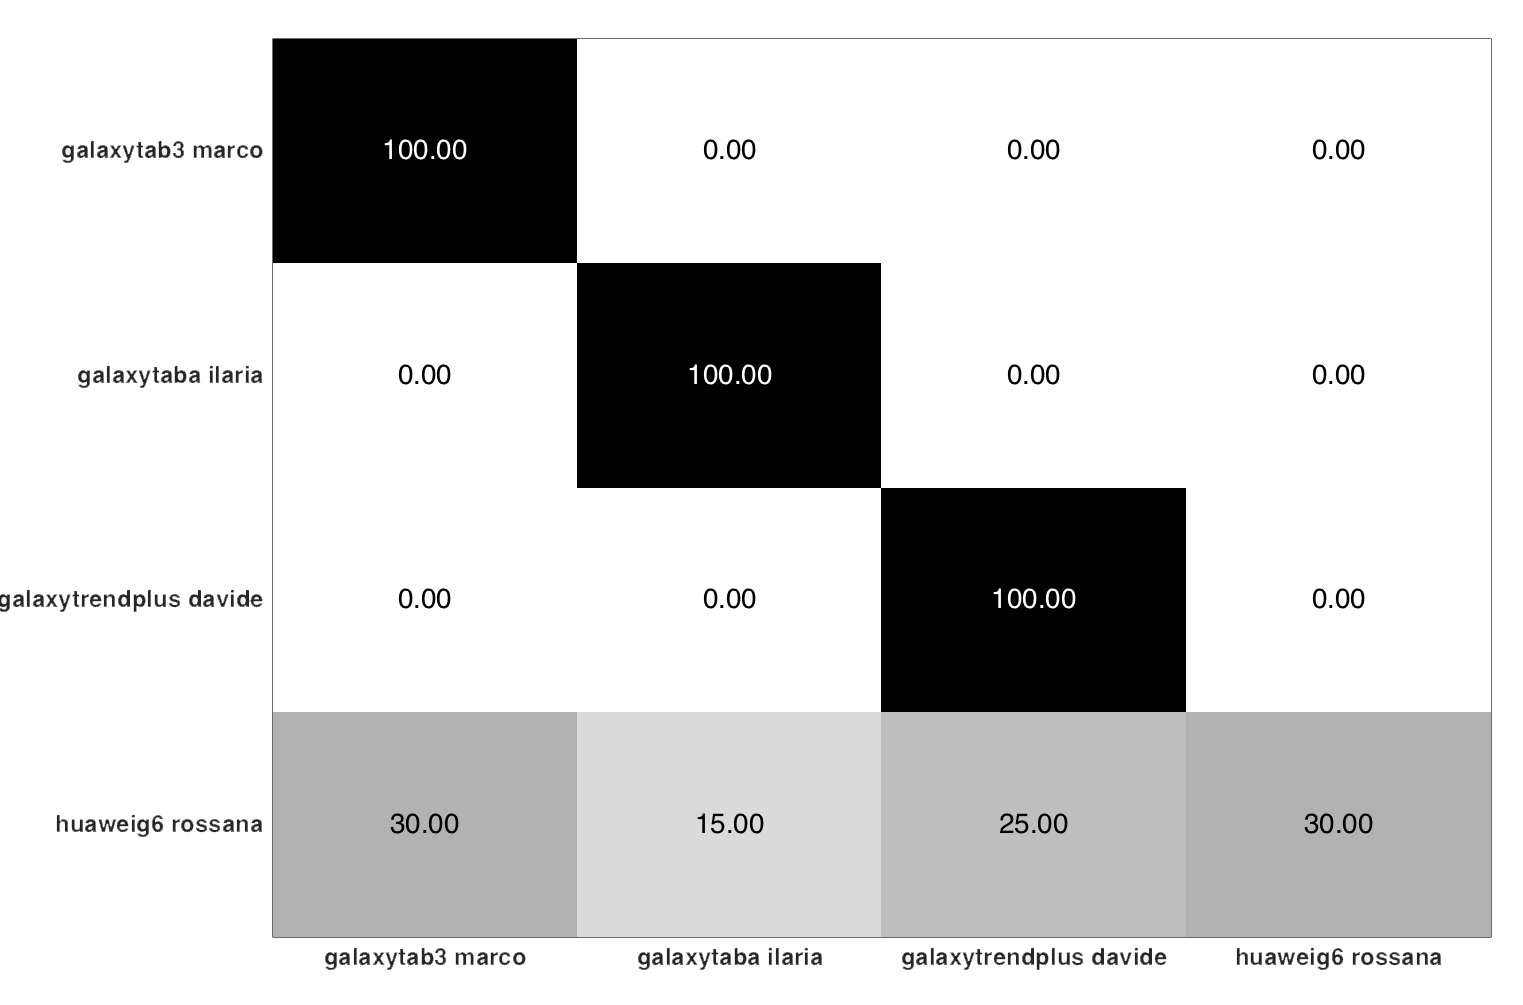
\includegraphics[width=0.4\textwidth]{images/confusionmatrix_nat_4.png}
\end{center}
  \caption{Matrice di confuzione per il caso delle immagini naturali usando 4 dispositivi.}
\label{fig:validation}
\end{figure}

\begin{figure}[h]
\begin{center}
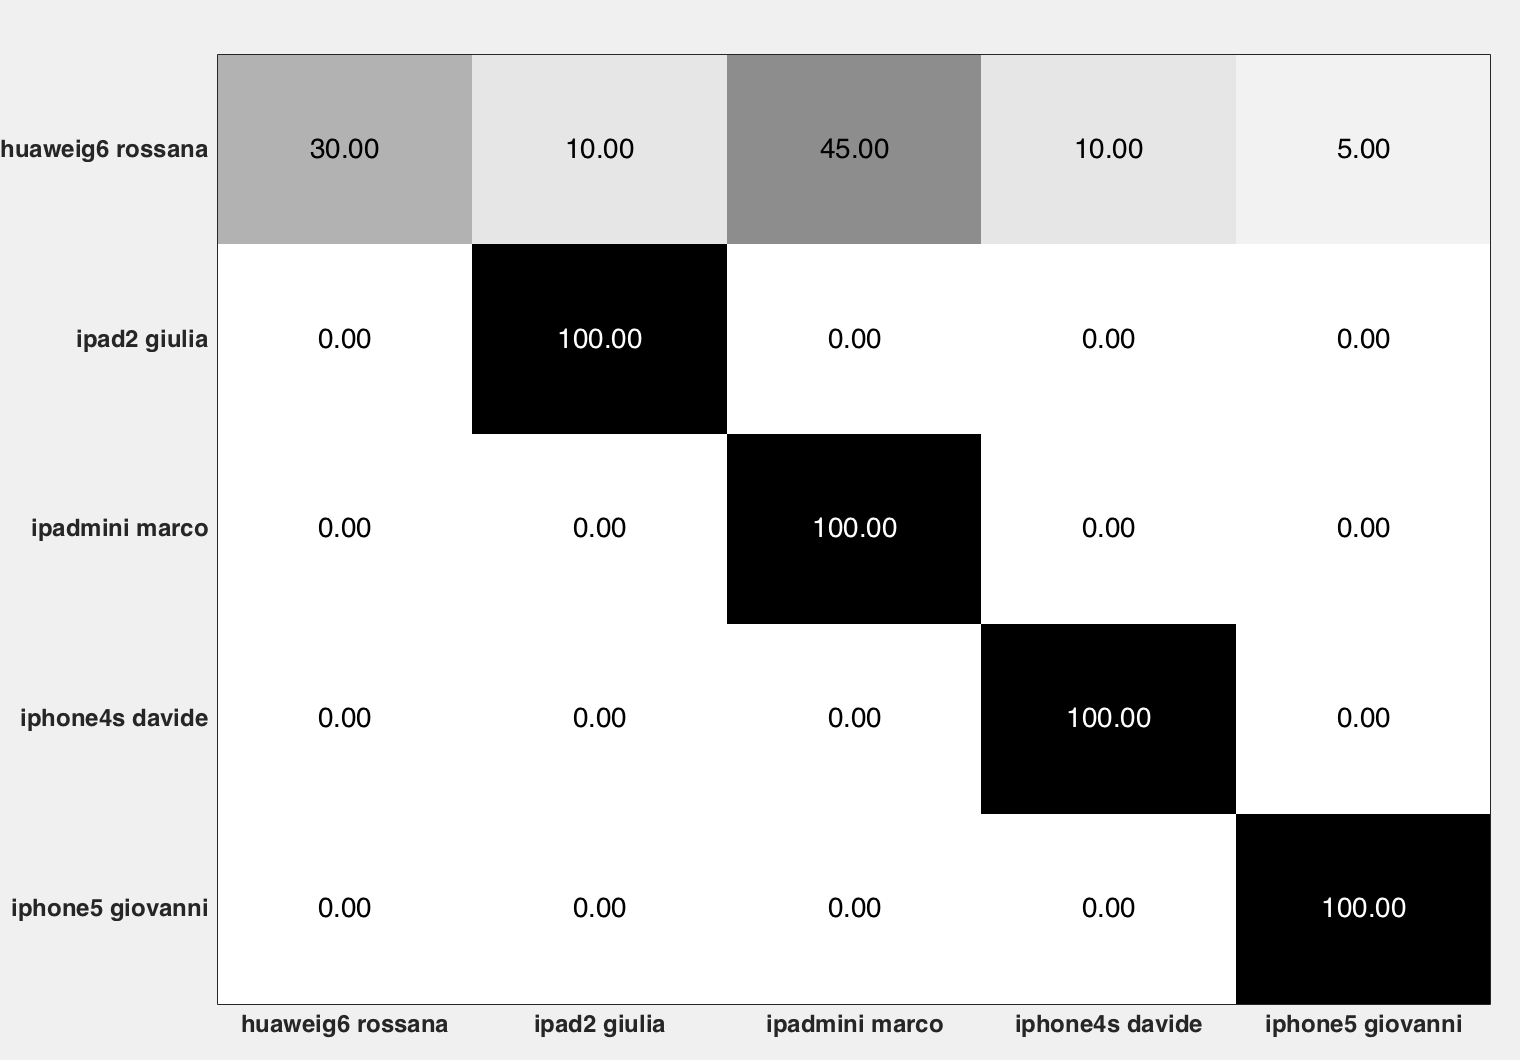
\includegraphics[width=0.4\textwidth]{images/confusionmatrix_nat_5.png}
\end{center}
  \caption{Matrice di confuzione per il caso delle immagini naturali usando 5 dispositivi.}
\label{fig:validation}
\end{figure}

\begin{figure}[h]
\begin{center}
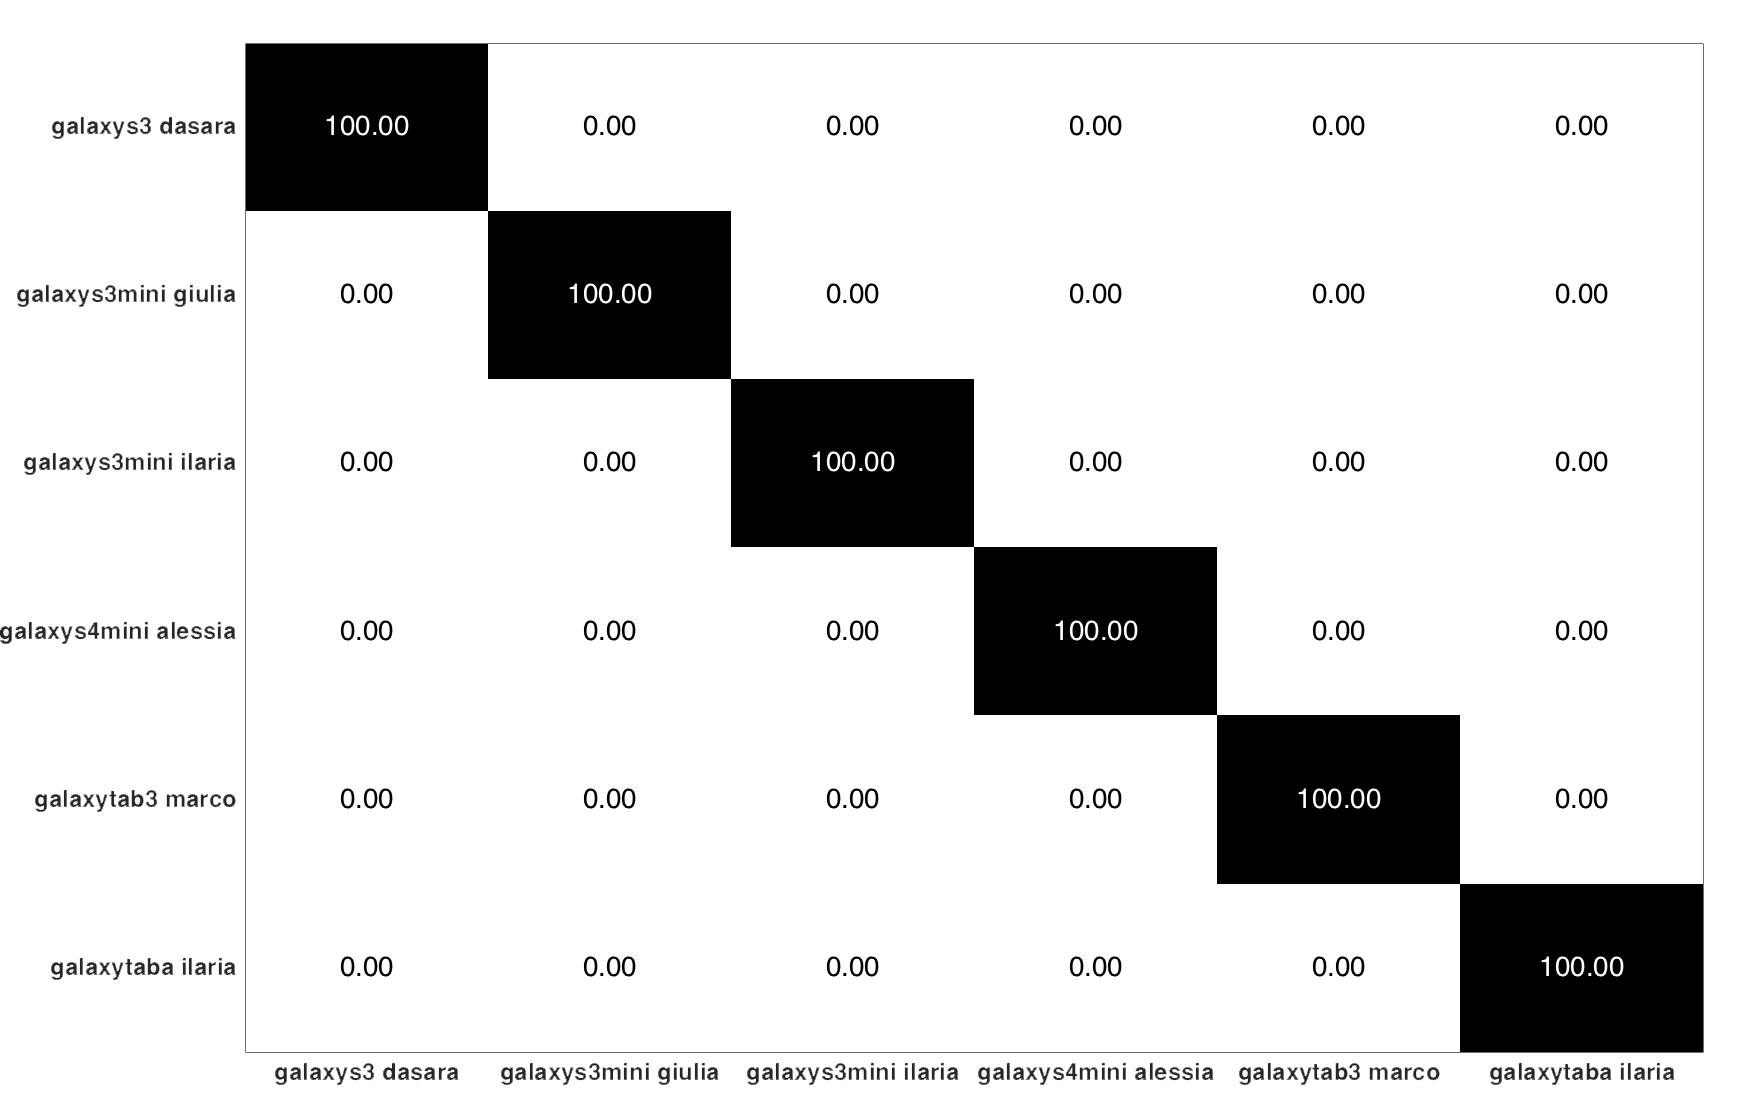
\includegraphics[width=0.4\textwidth]{images/confusionmatrix_nat_6.png}
\end{center}
  \caption{Matrice di confuzione per il caso delle immagini naturali usando 6 dispositivi.}
\label{fig:validation}
\end{figure}

Nel caso delle immagini naturali la validazione ottiene dei buoni risultati rispetto a tutte e tre le ripartizioni del dataset. Le immagini di validazione vengono associate alla giusta fingerprint con un'accuratezza del 100\% su tutti i dispositivi; l'unica eccezione è rappresentata dal dispositivo Huawei G6. Gli errori in questo caso non sono però dovuti ad una fingerprint rumorosa, poichè nella fase di clustering è stata ottenuta una percentuale di falsi positivi pari a 0. L'errore di classificazione è quindi dovuto in fase di validazione, ovvero quando, utilizzando la PCE viene calcolata la similitudine fra le immagini di test e le fingerprint estratte.

\begin{figure}[h]
\begin{center}
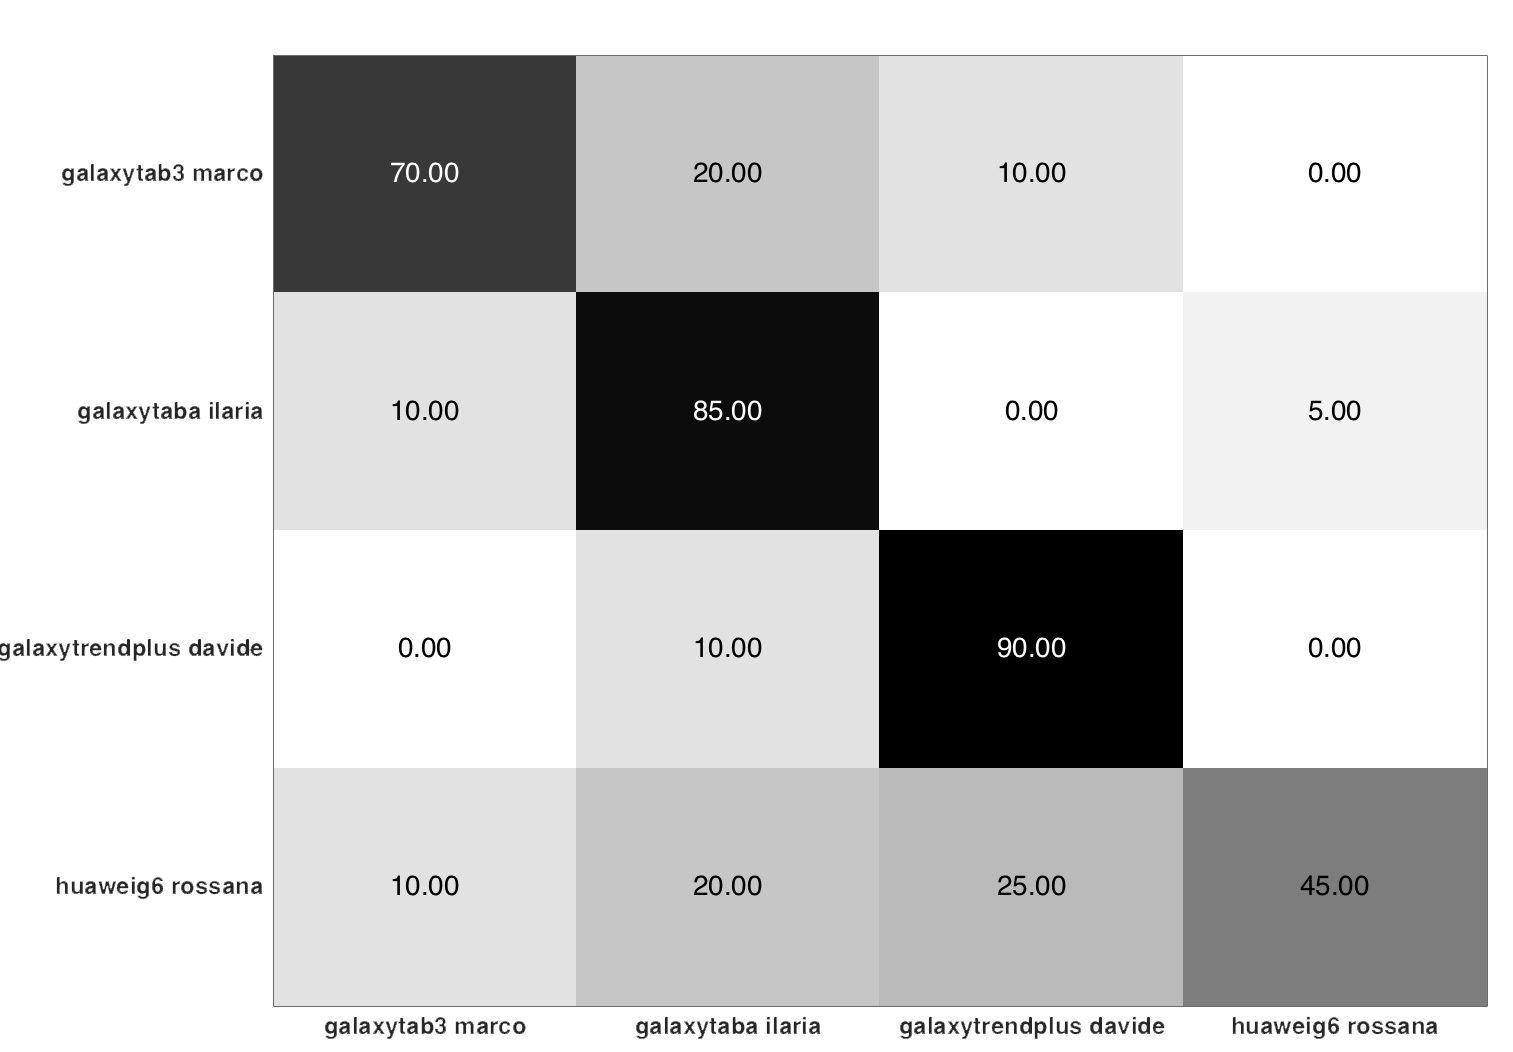
\includegraphics[width=0.4\textwidth]{images/confusionmatrix_fb_4.png}
\end{center}
  \caption{Matrice di confuzione per il caso delle immagini scaricati da Facebook usando 4 dispositivi.}
\label{fig:validation}
\end{figure}

\begin{figure}[h]
\begin{center}
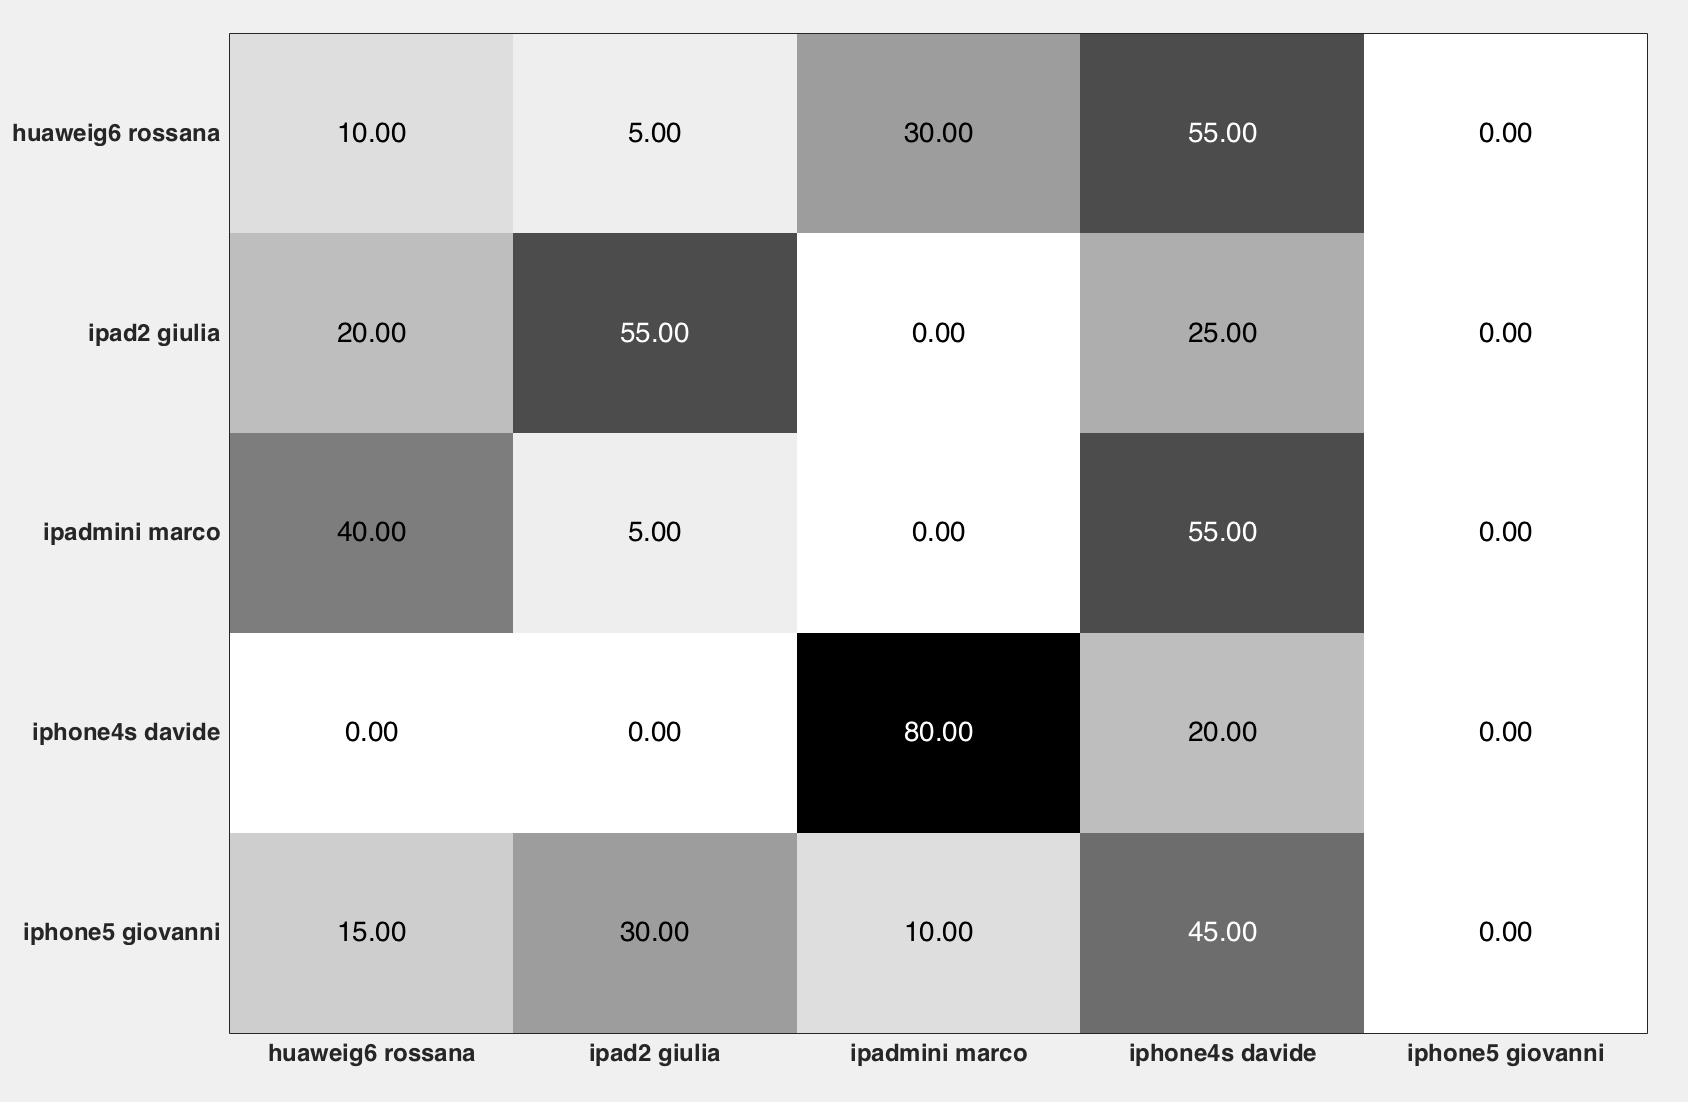
\includegraphics[width=0.4\textwidth]{images/confusionmatrix_fb_5.png}
\end{center}
  \caption{Matrice di confuzione per il caso delle immagini scaricati da Facebook usando 5 dispositivi.}
\label{fig:validation}
\end{figure}

\begin{figure}[h]
\begin{center}
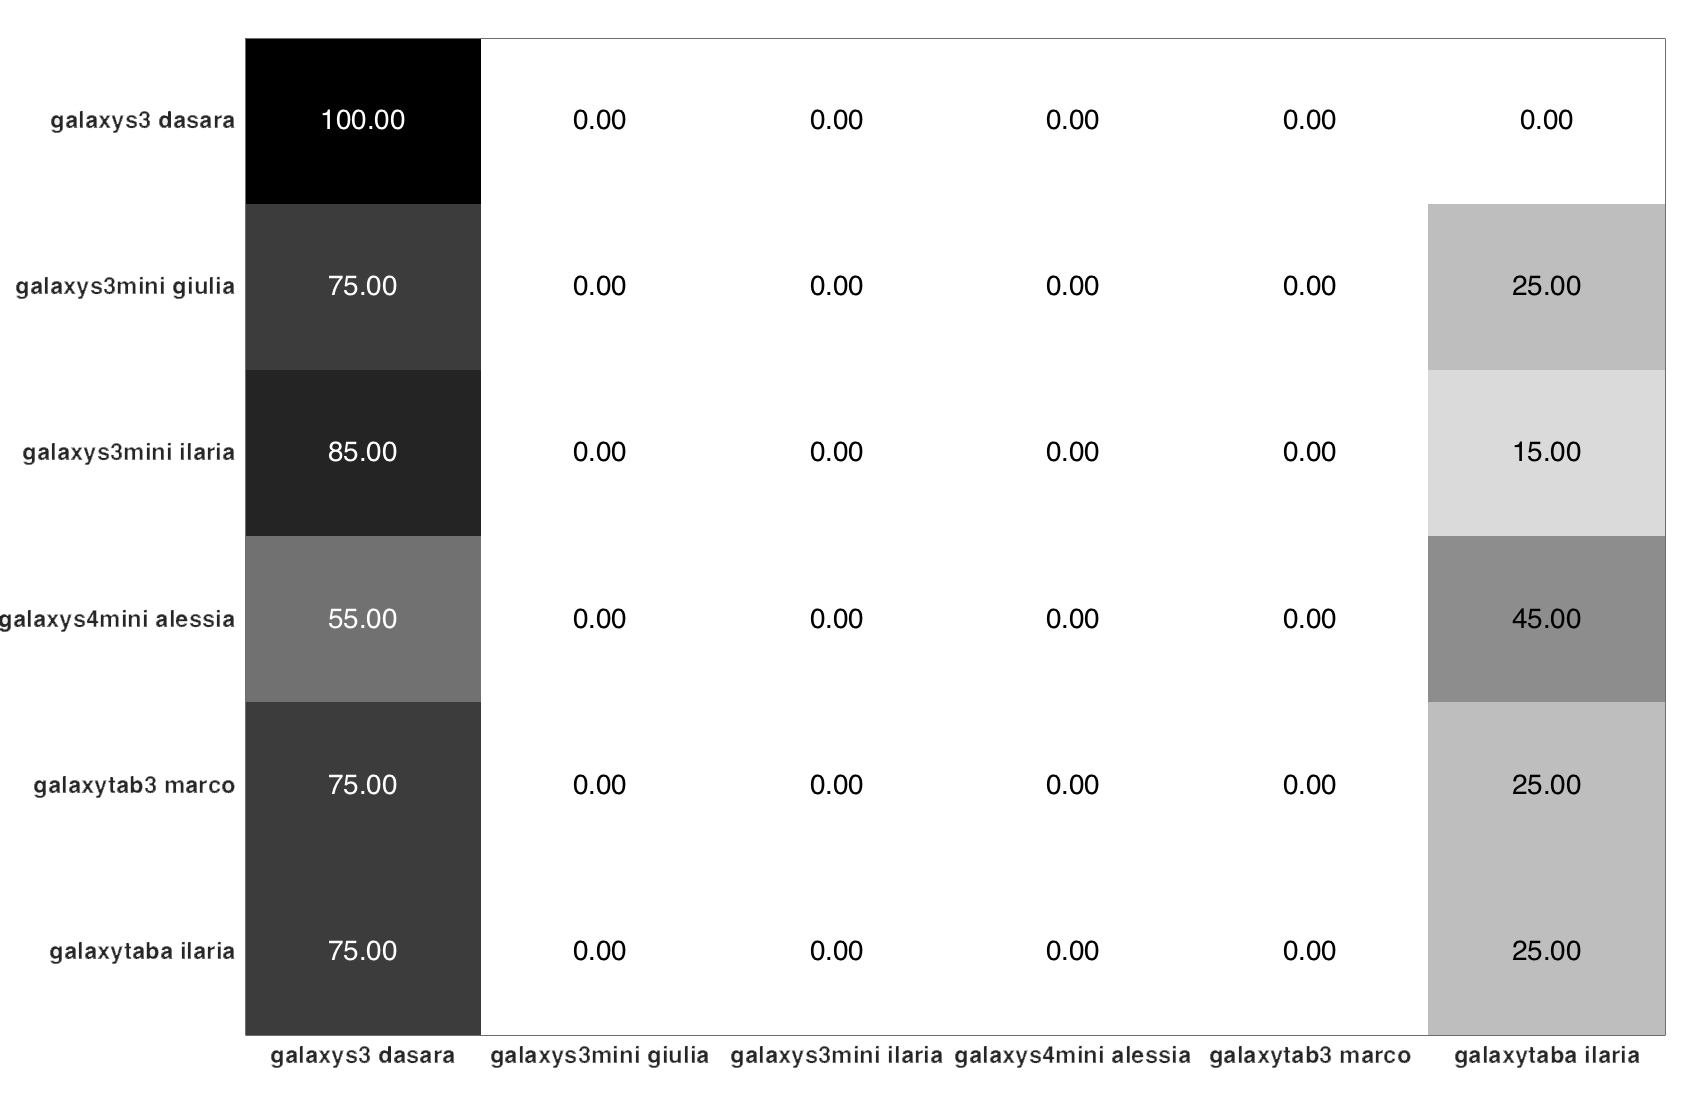
\includegraphics[width=0.4\textwidth]{images/confusionmatrix_fb_6.png}
\end{center}
  \caption{Matrice di confuzione per il caso delle immagini scaricati da Facebook usando 6 dispositivi.}
\label{fig:validation}
\end{figure}

Nel caso delle immagini scaricate da Facebook, i risultati sono inconcludenti. Solo l'insieme da 4 dispositivi, sempre ad eccezione del dispositivo Huawei G6, presenta valori accettabili. A differenza del precedente, in questo caso i molteplici errori di classificazione sono dovuti alla fase di clustering. Come mostrato nella sezione sulla selezione della soglie per il clustering, è difficile trovare una soglia che produca una clusterizzazione corretta e priva di falsi positivi, cosa che incide sulla qualità delle fingerprint. Inoltre, essendo tali immagini compresse rispetto a quelle naturali, queste perdono in informazione e così la PNRU estratta è meno significativa. Infatti i valori medi della matrice dei pesi, calcolati con la PCE,  in questo caso sono all'incirca di un ordine di grandezza inferiore rispetto ai valori medi della matrice dei pesi del caso delle immagini naturali. Ciò si ripercuote sulla soluzione dell'equazione che Normalized Cuts utilizza per partizionare il grafo.

Si può dedurre dai risultati che il nostro metodo di identificazione automatica dei dispositivi non è efficace per immagini che hanno subito una compressione, poichè le PNRU non sono sufficientemente discriminanti. Per quanto riguarda le immagini naturali, i risultati della validazione sono multo buoni ad eccezione di un unico dispositivo.
\section{Conclusioni}

In questo articolo abbiamo presentato un metodo di identificazione automatica di dispositivi a partire da un insieme di immagini la cui provenienza è ignota. Il metodo, prendendo le basi da \cite{ Amerini2014831} e apportandone alcune modifiche, funziona come segue:
\begin{enumerate}
\item Le PRNU vengono estratte dalle immagini del dataset. 
\item Per ogni coppia di PRNU viene calcolata una misura di similarità utilizzando la PCE e viene costruita una matrice dei pesi che rappresenta il grafo completamente connesso.
\item L'algoritmo Normalized Cuts partiziona il grafo e divide le immagini in clusters.
\item Per ogni clusters viene calcolata una fingerprint che rappresenta un dispositivo, a partire dalle PRNU delle immagini appartenenti a tale cluster.
\item Infine una fase di validazione che verifica la qualità delle fingerprint estratte.
\end{enumerate}

Il dataset utilizzato contiene immagini direttamente acquisite dai dispositivi e le stesse immagini caricate e poi scaricate da Facebook. I risultati ottenuti nella fase di validazione differiscono a seconda del tipo di immagini utilizzate. Le fingerprints estratte per il caso delle immagini naturali sono di qualità ed il metodo è in grado di associare una generica immagine del dataset alla fingerprint corretta, ad eccezione per le immagini provenienti dal dispositivo Huawei.

Per quanto riguarda le immagini scaricate da Facebook, il metodo si è mostrato meno efficace. Questo è dovuto alla fatto che le immagini caricate su un social network subiscono, in genere, una compressione che va peggiorare la qualità delle PRNU estratte. Questo ha conseguenze sulla misura di similarità, in questo caso la PCE. La similarità fra immagini provenienti dallo stesso dispositivo risulta meno forte rispetto a considerare la similarità delle stesse immagini per il caso delle immagini naturali. Inoltre a causa di ciò, la fase di clustering produce un numero maggior di clusters che, seppur puliti, conterranno un numero minore di immagini rispetto al caso delle immagini naturali, a causa di una TPR molto più bassa; tutto ciò va ad influire sulla qualità delle fingerprints nella fase di validazione. Va notato comunque, che la compressione, perlomeno quella effettuata da Facebook, sembra incidere maggiormente su alcuni dispositivi piuttosto che su altri, con alcuni di questi che infatti ottengono un'accuratezza nella predizione alta indipendentemente dalla ripartizione del dataset in cui si ritrovano, come mostrato nelle matrici di confusione dei vari esperimenti.

In conclusione, il metodo implementato funziona correttamente quando si estraggono delle PRNU di qualità dalle immagini, ovvero pulite e calcolate con tante immagini, cosa meno possibile se l'immagine è stata sottoposta ad una pesante compressione.

%-------------------------------------------------------------------------

{\small
\bibliographystyle{ieee}
\bibliography{egbib}
}

\end{document}
